\documentclass[wide,a4paper,titlepage,12pt]{article}
\usepackage{polski}
\usepackage[utf8]{inputenc}
\usepackage{setspace}
\usepackage{graphicx}

\title{Rozproszona aplikacja umożliwiająca przeglądanie fraktali}
\author{Tymon Tobolski {\small(181037)}\\ Jacek Wieczorek {\small(181043)} \\
Mateusz Lenik {\small(181142)}}

\makeatletter
\renewcommand{\maketitle}{
  \begin{titlepage}
    \begin{center}
      \vspace*{3cm}
      \LARGE \@title \par
      \vspace{2cm}
      \textit{\small Autor:}\par
      \normalsize \@author\par \normalsize
      \vspace{3cm}
      \textit{\small Prowadzący:}\par
      dr inż. Marek Woda \par
      \vspace{2cm}
      Wydział Elektroniki\\ III rok\\ Pn 12.15 - 14.00\par

    \end{center}
  \end{titlepage}
}
\makeatother
\setlength{\parindent}{0em}
\onehalfspacing

\begin{document}
\maketitle
\tableofcontents
\newpage

\section{Opis projektu}
\paragraph{}
Celem projektu jest stworzenie aplikacji internetowej pozwalającej użytkownikowi
na przeglądanie fraktali renderowanych na klastrze. Aplikacja
pozwalałaby na przybliżanie i oddalanie widocznej części fraktala, zmianę
kolorów oraz zapisywanie ostatniej przeglądanej pozycji przez danego
użytkownika.

\section{Uzasadnienie biznesowe}
\paragraph{}
Projekt może zostać wykorzystany jako proof of concept dla aplikacji
przetwarzających duże ilości danych i prezentację ich w formie lub na mapie.
Jest to proste do rozbudowy demo technologiczne, na podstawie którego można
stworzyć bardziej skomplikowane aplikacje.

\section{Technologie}
\paragraph{}
Aplikacja będzie oparta o technologie wykorzystujące JVM, dzięki czemu możliwe
będzie uruchomienie jej na kilku platformach bez konieczności modyfikacji.
Dodatkowo ułatwia to korzystanie z różnych języków programowania podczas
implementacji aplikacji. Za interfejs webowy będzie odpowiadała aplikacja w Ruby
on Rails, która będzie się komunikowała z rozproszonym backendem
zaimplementowanym w Scali.

\begin{itemize}
  \item Platforma: JVM
  \item Język implementacji: Ruby, Scala, CoffeeScript
  \item Baza danych: SQLite lub MySQL
  \item Framework: Ruby on Rails
\end{itemize}

\newpage
\section{Funkcjonalności systemu}

\begin{itemize}
  \item Obsługa użytkowników
    \begin{itemize}
      \item Utworzenie konta,
      \item Autentykacja za pomocą OAuth,
      \item Pobieranie awatarów,
      \item Zapisanie ustawień i ostatniej przeglądanej pozycji.
    \end{itemize}
  \item Wyświetlanie mapy
    \begin{itemize}
      \item Nawigacja po mapie za pomocą myszy,
      \item Wybór renderowanego fraktala,
      \item Wybór kolorów dla renderowanego fraktala,
      \item Wybór metody podziału obrazu do renderowania.
    \end{itemize}
  \item Renderowanie
    \begin{itemize}
      \item Podział obrazu na mniejsze fragmenty do renderowania na backendzie,
      \item Przesyłanie żądań z aplikacji do backendu,
      \item Komunikacja między węzłami backendu.
    \end{itemize}
\end{itemize}

\section{Implementacja}
\paragraph{}
Praca nad projektem została podzielona na dwie części, aplikację internetową
oraz rozproszone API pozwalające na renderowanie części fraktala.

W obecnej wersji system pozwala na wybór renderowanego fraktala spośród dwóch algorytmów,
Mandelbrota i zbioru Julii. Oba obrazy można uzyskać zarówno w wersji monochromatycznej, 
jak i kolorowej. Dla każdego z fraktali można również zdefiniować ilość iteracji algorytmu oraz
wymiary płytek. 

\section{Aplikacja internetowa}
\paragraph{}
Aplikacja internetowa została utworzona przy użyciu frameworka Ruby on Rails. Do
wyświetlania fraktala wykorzystana została biblioteka Leaflet. Aplikacja
pobiera poszczególne części fraktala łącząc się z rozproszonym API. Obecnie
zaimplementowane jest logowanie za pomocą Twitter OAuth. Dla zalogowanego
użytkownika zapisywana jest ostatnie przeglądane współrzędne oraz wybrane parametry renderowanego fraktala.

\paragraph{}
Aplikacja internetowa została zaimplementowana w architekturze MVC z wykorzystaniem architektury REST.

\subsection{Kontrolery}
\subsubsection{PagesController}
\paragraph{}
Kontroler odpowiedzialny za wyświetlanie stron statycznych.

\subsubsection{SessionsController}
\paragraph{}
Kontroler odpowiedzialny za tworzenie i kończenie sesji użytkownika

\subsubsection{UsersController}
\paragraph{}
Kontroler odpowiedzialny za aktualizację ustawień fraktala dla zalogowanego użytkownika

\subsection{Widoki}
\paragraph{}
Wszelkei widoki zostały napisane przy uzyciu języka znaczników \textit{Haml}. W celu generowania 
formularzy użyty został gem \textit{SimpleForm}, a cały layout oparty o bibliotekę styli 
css - \textit{Bootstrap}. Skrypty wykorzystujące \textit{jQuery}, napisane zostały przy pomocy 
języka \textit{CoffeScript}, kompilowalnego do kodu javascript.

\subsection{Model}
\paragraph{}
W aplikacji zstał wykorzystany model \textit{User} przechowujący podstawowe dane o zarejestrowanych użytkownikach,
a także ich ustawienia fraktali.

\section{Rozproszone API}
\paragraph{}
Biblioteka Leaflet pobiera z API obrazki o zdefiniowanych przez użytkownika rozmiarach w pikselach
korzystając z URL w formacie \texttt{http://\{serwer\}/img/\{x\}/\{y\}/\{z\}}
wypełniając pola \texttt{x}, \texttt{y}, \texttt{z} odpowiednimi
wartościami. Następnie, zgodnie z rysunkiem \ref{fig:loadbalancing}, zapytanie
jest przydzielane do odpowiednich węzłów, renderowane, a rezultat
zwracany jest do klienta.

\begin{figure}[h!]
\begin{center}
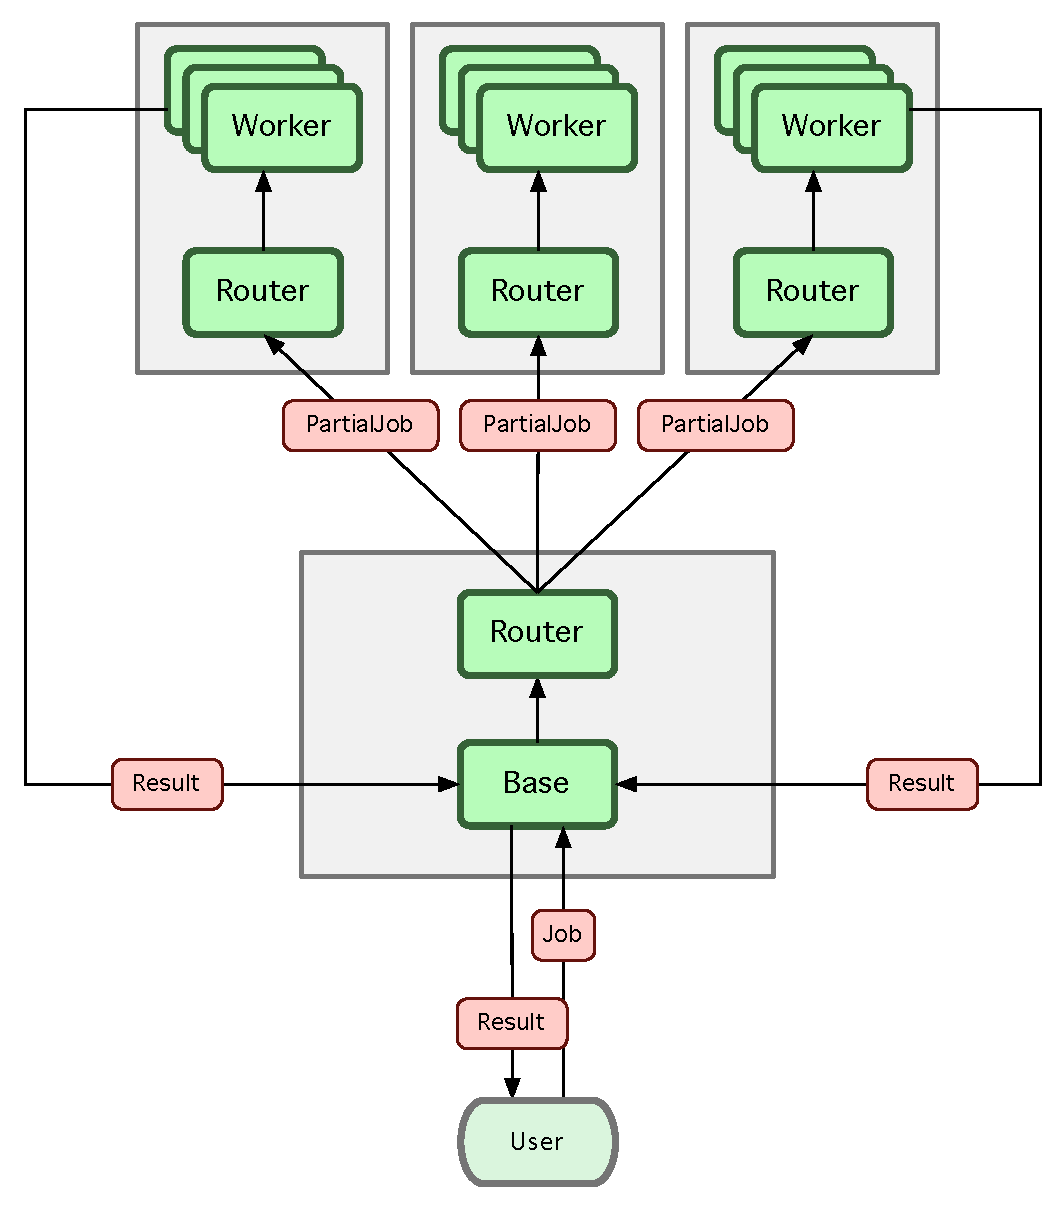
\includegraphics[scale=0.5]{schema.pdf}
\end{center}
\caption{Load balancing.}
\label{fig:loadbalancing}
\end{figure}

API zostało zaimplementowane w języku Scala wykorzystując bibliotekę Akka.io
umożliwiającą łatwe użycie Actor pattern.

\section{Wdrożenie}
\paragraph{}
Aplikacja została wdrożona na klastrze obliczeniowym składającym się z
dziewięciu maszyn wirtualnych. Ze względu na łatwą konfigurację, jako host
maszyn wirtualnych została wybrana platforma Amazon EC2.

\begin{figure}[h!]
\begin{center}
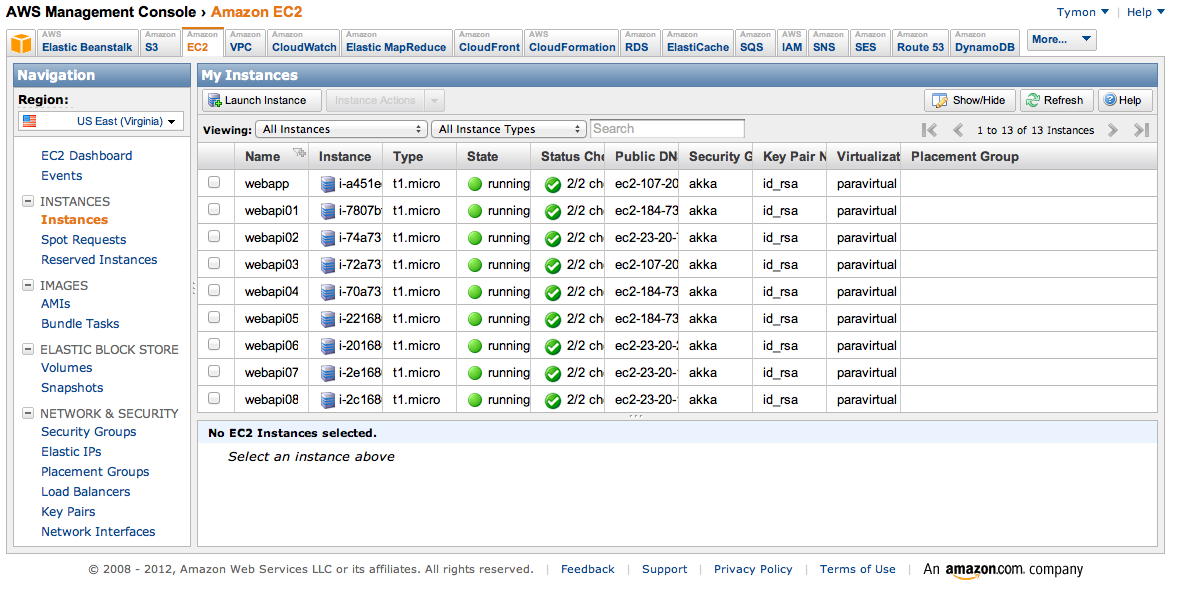
\includegraphics[scale=0.33]{ec2.png}
\end{center}
\caption{Klaster obliczeniowy.}
\label{fig:ec2}
\end{figure}

\section{Testy}
\paragraph
TODO

\section{Podsumowanie}
\paragraph{}
Zaimplementowana zostały podstawowe funkcjonalności aplikacji. W przyszłości
dodane zostaną pozostałe funkcjonalności, takie jak wybór dodatkowych opcji w
aplikacji. Do projektu dodana zostanie również dokumentacja projektowa oraz
testy behawioralne.

\end{document}

